\documentclass[11pt,letterpaper]{article}
\usepackage{fontspec}
\setmainfont{texgyrepagella}[Extension=.otf,UprightFont=*-regular,BoldFont=*-bold,ItalicFont=*-italic,BoldItalicFont=*-bolditalic]
\usepackage[bidi=default]{babel}
\babelprovide[import,main]{spanish}
\babelprovide[import]{hebrew}
\babelprovide[import]{ancientgreek}
\babelfont[hebrew]{rm}[Path=fonts/,BoldFont=NotoHebrewSerif-700.ttf,Scale=0.95]{NotoHebrewSerif-400.ttf}
\babelfont[ancientgreek]{rm}[Path=fonts/]{GFSPorson.otf}
\newcommand{\heb}[1]{\mbox{\foreignlanguage{hebrew}{#1}}}
\newcommand{\grc}[1]{\foreignlanguage{ancientgreek}{#1}}
\usepackage{needspace}
\newcommand{\hebverso}[1]{\par\needspace{7\baselineskip}\smallskip{\centering\begin{otherlanguage}{hebrew}\large #1\end{otherlanguage}\par}\smallskip}
\usepackage[margin=2.5cm,headheight=14pt]{geometry}
\usepackage{microtype,ragged2e,booktabs,graphicx,xcolor,csquotes,array}
\usepackage[hidelinks]{hyperref}\usepackage{xurl}\urlstyle{same}
\usepackage[most]{tcolorbox}
\usepackage{tikz}\usetikzlibrary{arrows.meta,positioning,calc,decorations.pathreplacing}
\usepackage{titlesec,fancyhdr,extramarks}
% Paleta "Israel": celeste y azul del tejelet (Nm 15:38) con oro del santuario
% (nombres conservados por compatibilidad: ladrillo = azul tejelet, cafe = azul real, cafeosc = azul noche,
%  piedra = celeste claro, sepia = azul pizarra)
\definecolor{cafe}{RGB}{26,82,150}\definecolor{cafeosc}{RGB}{11,33,74}\definecolor{tinta}{RGB}{20,32,56}
\definecolor{oro}{RGB}{206,162,52}\definecolor{ladrillo}{RGB}{20,68,140}
\definecolor{piedra}{RGB}{234,243,251}\definecolor{sepia}{RGB}{72,102,140}\definecolor{celeste}{RGB}{96,166,222}
\titleformat{\section}{\Large\bfseries\color{ladrillo}}{\thesection.}{0.6em}{}
\titleformat{\subsection}{\large\bfseries\color{cafe}}{\thesubsection}{0.6em}{}
\pagestyle{fancy}\fancyhf{}
\fancyhead[L]{\foreignlanguage{spanish}{\small\itshape\color{sepia}\firstleftmark}}\fancyhead[R]{\foreignlanguage{spanish}{\small\color{sepia}\thepage}}
\renewcommand{\sectionmark}[1]{\markboth{#1}{}}
\setlength{\parindent}{1.27cm}\linespread{1.15}\setlength{\emergencystretch}{3em}
\newtcolorbox{cita}[1][]{enhanced,colback=piedra,colframe=oro!90!ladrillo,boxrule=0pt,leftrule=2.5pt,arc=0pt,
  left=8pt,right=8pt,top=5pt,bottom=5pt,before skip=8pt,after skip=8pt,fontupper=\itshape,#1}
\newcommand{\fuente}[1]{\par\hfill{\upshape\bfseries\small\textcolor{ladrillo}{#1}}}
\newtcolorbox{nota}[1][]{enhanced,colback=oro!12,colframe=oro!80!ladrillo,boxrule=0.6pt,arc=2pt,
  fonttitle=\bfseries\small,coltitle=cafe,colbacktitle=oro!35,fontupper=\small,title={#1}}
\newcommand{\refapa}[1]{\par{\RaggedRight\hangindent=1.27cm\hangafter=1\noindent #1\par}\vspace{4pt}}
\newcommand{\destacar}[1]{\textbf{\textcolor{ladrillo}{#1}}}
\providecommand{\pt}[2]{({#1-30},{#2-29})}
\title{\color{ladrillo}\bfseries De Cristo a la destrucción del templo\\[4pt]\large\color{cafe}\mdseries El Mesías de Israel, un remanente que cree y un juicio que lleva escrito su «hasta»}
\author{}\date{\color{sepia}Serie «Israel, el pueblo de Dios» · Estudio 7}
\begin{document}
\maketitle\thispagestyle{empty}

\begin{abstract}\noindent
Este séptimo estudio recorre la historia de Israel desde el nacimiento de Jesús hasta la caída del Segundo Templo y de Masada, y muestra que los mismos textos que anuncian la ruina de Jerusalén le fijan un término y apuntan a la restauración de Israel. Jesús vive dentro de las fiestas, el templo y los profetas de su pueblo y asume la figura del siervo de Isaías llamado a «levantar las tribus de Jacob» y a ser «luz de las naciones» (Is 49:6); en torno a él se forma un remanente judío creyente, núcleo del pueblo restaurado, al que los gentiles se suman sin ocupar su lugar. La destrucción del año 70, anunciada con palabras de Jeremías, se lee como un juicio dentro del pacto que lleva escrito su «hasta»: «hasta que digáis: Bendito el que viene» (Mt 23:39), «hasta que los tiempos de los gentiles se cumplan» (Lc 21:24), «hasta los tiempos de la restauración» (Hch 3:21). Al relato bíblico se suman Josefo, la arqueología de Jerusalén y Masada y la respuesta rabínica de Yavne y de Tisha be-Av. Pablo, que escribe antes de esa fecha, ya había dejado dicho que «no ha desechado Dios a su pueblo» (Ro 11:2), y desde ahí arranca el Estudio~8.
\par\smallskip\noindent\textbf{Palabras clave:} Mesías, remanente, nuevo pacto, Segundo Templo, guerra judía, Yavne, Tisha be-Av, restauración, Romanos 11.
\end{abstract}

\section{Introducción}

¿Qué significa para Israel que su templo fuera destruido cuarenta años después de la crucifixión de Jesús? Una respuesta muy extendida en la historia de la iglesia ve en el año 70 la prueba de que Dios rechazó a Israel y entregó sus promesas a otro pueblo; otra, habitual en lecturas modernas, desliga a Jesús de la historia de los suyos. El Nuevo Testamento no sostiene ninguna de las dos. Jesús nace «bajo la ley» (Gá 4:4), elige a doce, enseña en las fiestas y llora sobre Jerusalén antes de anunciar su ruina, y sus seguidores judíos siguen orando en el templo hasta poco antes de la guerra.

En su persona asume el llamado de Israel, como Hijo llamado de Egipto (Mt 2:15; Os 11:1), como siervo que restaura a las tribus y alumbra a las naciones (Is 49:5–6) y como quien establece el nuevo pacto prometido «a la casa de Israel y a la casa de Judá» (Jer 31:31 [31:30]). A su alrededor surge un remanente judío creyente al que luego se suman los gentiles. La caída del templo se comprende entonces a la luz de la del 586 a.\,e.\,c., que Jeremías anunció en el mismo libro donde juró la permanencia de Israel: un juicio dentro del pacto, cuyos textos llevan un «hasta» que mira hacia la restauración que Pablo desarrollará en Romanos 11.

\begin{nota}[Sobre traducción, numeración y fechas]
Traducción propia desde BHS y NA28; la LXX según Rahlfs-Hanhart. La numeración hebrea, cuando difiere, va entre corchetes. En esta etapa el reino del norte ya no existe y «Israel» designa casi siempre al pueblo entero; se indica cuando un texto evoca a las tribus del norte.
\end{nota}

\section{Marco cronológico}

Jesús nace en los días de Herodes el Grande (Mt 2:1), muerto en el 4 a.\,e.\,c., y Juan predica en el año quince de Tiberio (Lc 3:1), hacia el 28--29 e.\,c. La crucifixión ocurrió bajo Poncio Pilato, y la combinación del calendario pascual de los evangelios con los datos astronómicos deja el 30 o el 33 como fechas más probables. Siguen el concilio de Hch 15 (c. 48--49), la carta a los Romanos (c. 57), la muerte de Jacobo (62), la revuelta (66), la caída del templo (70) y la de Masada, que Josefo no fecha y que varios historiadores sitúan en el 74 en vez del 73 (Mason, 2016).

\begin{center}
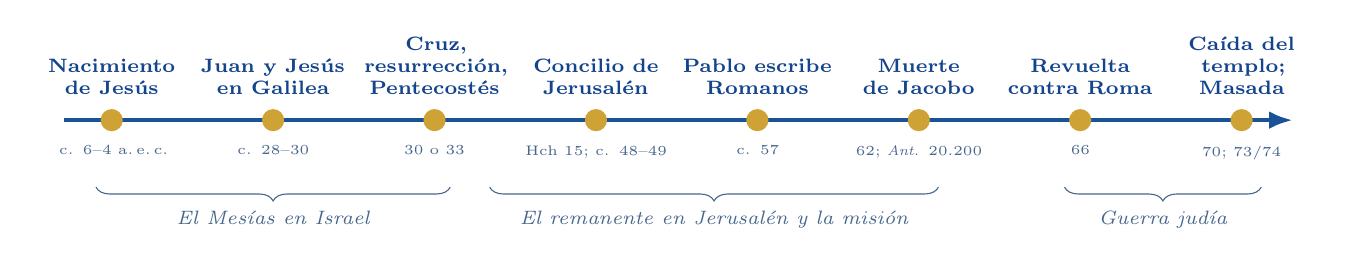
\begin{tikzpicture}[x=1cm,y=1cm]
\draw[line width=1.6pt,cafe,-{Latex[length=3mm]}] (0,0) -- (15.6,0);
\foreach \x/\t/\b in {0.6/{Nacimiento de Jesús}/{c. 6--4 a.\,e.\,c.},
                      2.65/{Juan y Jesús en Galilea}/{c. 28--30},
                      4.7/{Cruz, resurrección, Pentecostés}/{30 o 33},
                      6.75/{Concilio de Jerusalén}/{Hch 15; c. 48--49},
                      8.8/{Pablo escribe Romanos}/{c. 57},
                      10.85/{Muerte de Jacobo}/{62; \emph{Ant.} 20.200},
                      12.9/{Revuelta contra Roma}/{66},
                      14.95/{Caída del templo; Masada}/{70; 73/74}}{
  \fill[oro] (\x,0) circle (4pt);
  \node[above,font=\scriptsize\bfseries,text=ladrillo,text width=1.9cm,align=center] at (\x,0.2) {\t};
  \node[below,font=\tiny,text=sepia,text width=1.8cm,align=center] at (\x,-0.2) {\b};}
\draw[decorate,decoration={brace,amplitude=5pt,mirror},sepia] (0.4,-0.85) -- (4.9,-0.85) node[midway,below=5pt,font=\scriptsize\itshape]{El Mesías en Israel};
\draw[decorate,decoration={brace,amplitude=5pt,mirror},sepia] (5.4,-0.85) -- (11.1,-0.85) node[midway,below=5pt,font=\scriptsize\itshape]{El remanente en Jerusalén y la misión};
\draw[decorate,decoration={brace,amplitude=5pt,mirror},sepia] (12.7,-0.85) -- (15.2,-0.85) node[midway,below=5pt,font=\scriptsize\itshape]{Guerra judía};
\end{tikzpicture}\\[2pt]
{\footnotesize\color{sepia}\textit{Nota.} Elaboración propia. Fechas aproximadas; el año de la crucifixión y el de la caída de Masada están en debate (véase el texto).}
\end{center}


\section{Contexto histórico y arqueológico}

Herodes, rey vasallo de Roma, reconstruyó el templo en una obra que seguía en curso en tiempos de Jesús (Jn 2:20). Desde el 6 e.\,c. Judea quedó bajo prefectos romanos, y el sumo sacerdote, nombrado por Roma o por los herodianos, presidía el sanedrín junto a fariseos, saduceos, esenios y la «cuarta filosofía» de los rebeldes (\emph{Ant.} 18.23).

\begin{center}\begin{minipage}[b]{0.24\linewidth}\centering
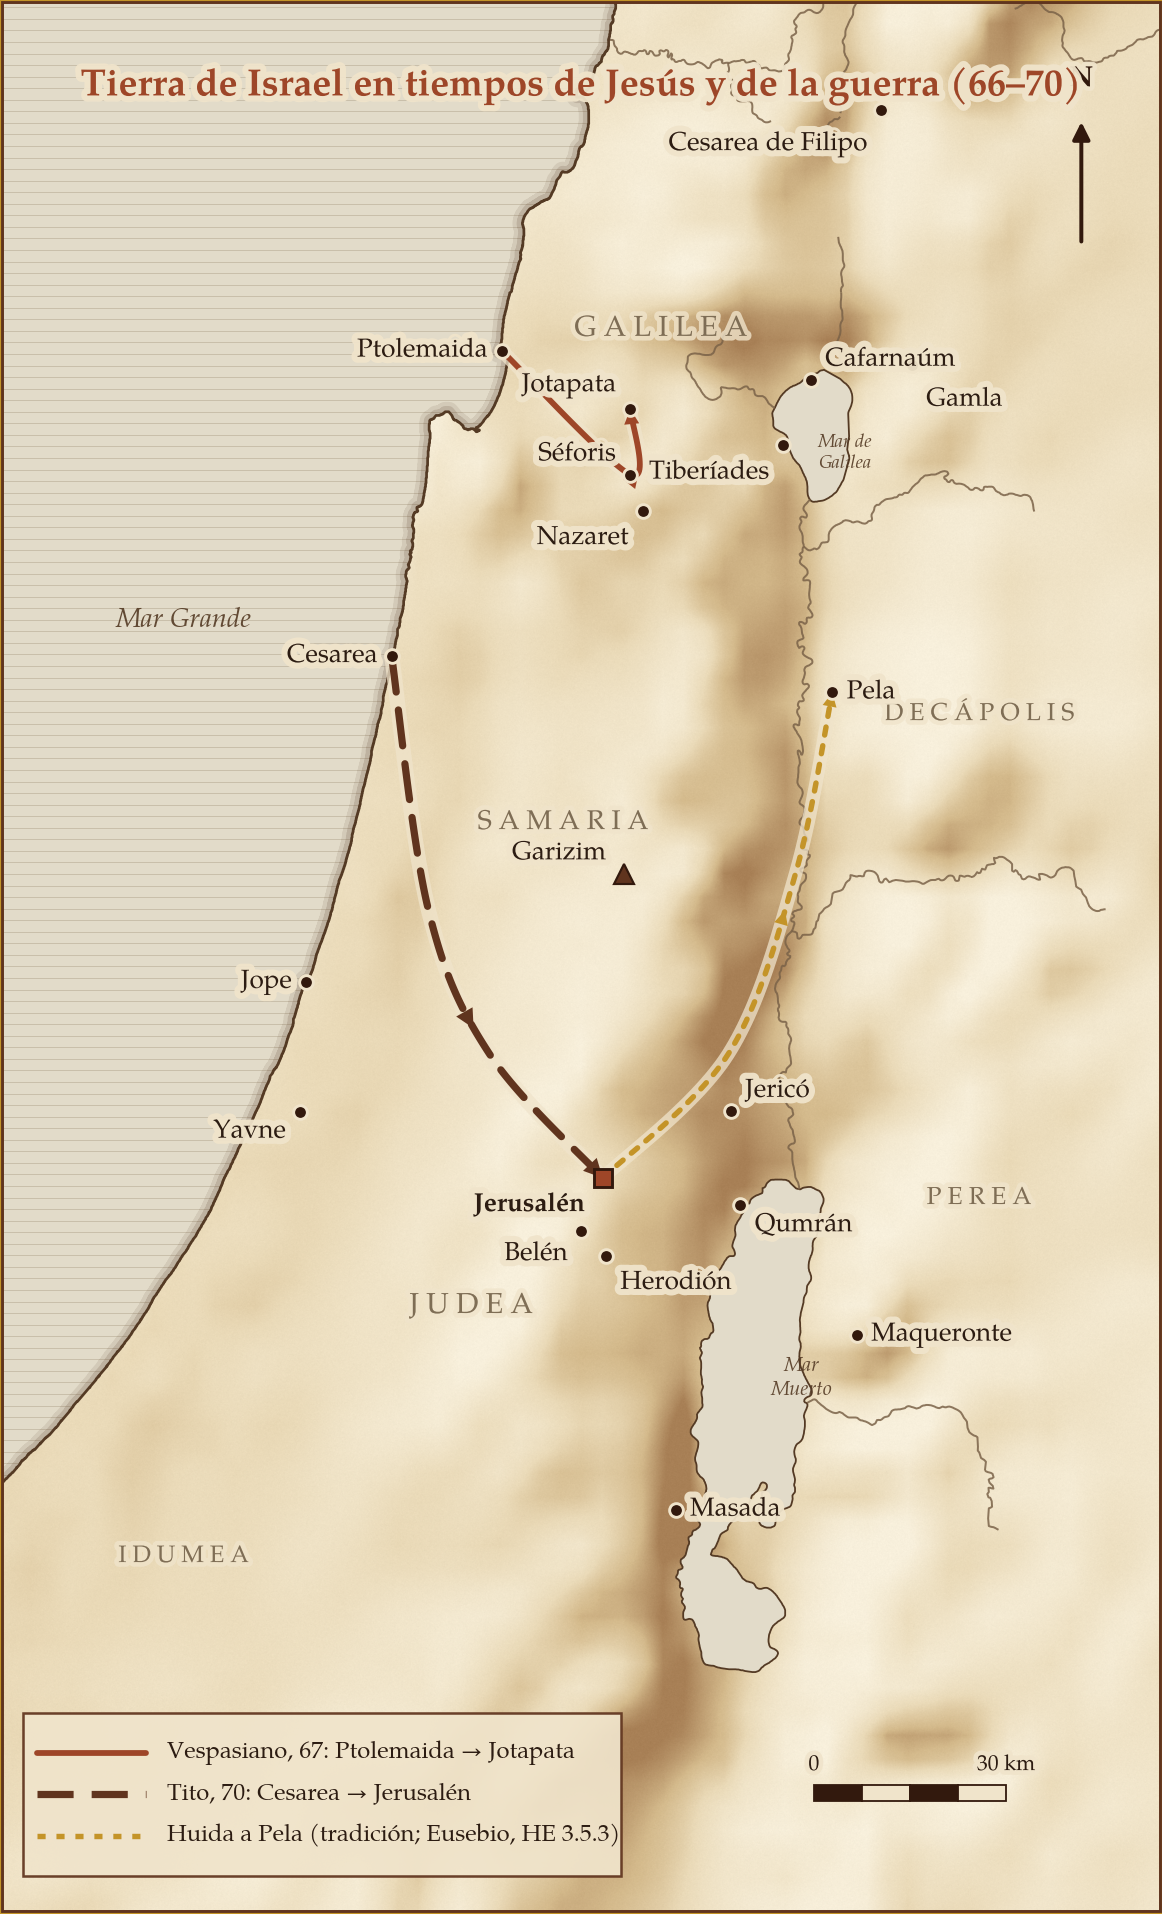
\includegraphics[width=\linewidth]{mapa_galilea.png}
\end{minipage}\hfill\begin{minipage}[b]{0.73\linewidth}\centering
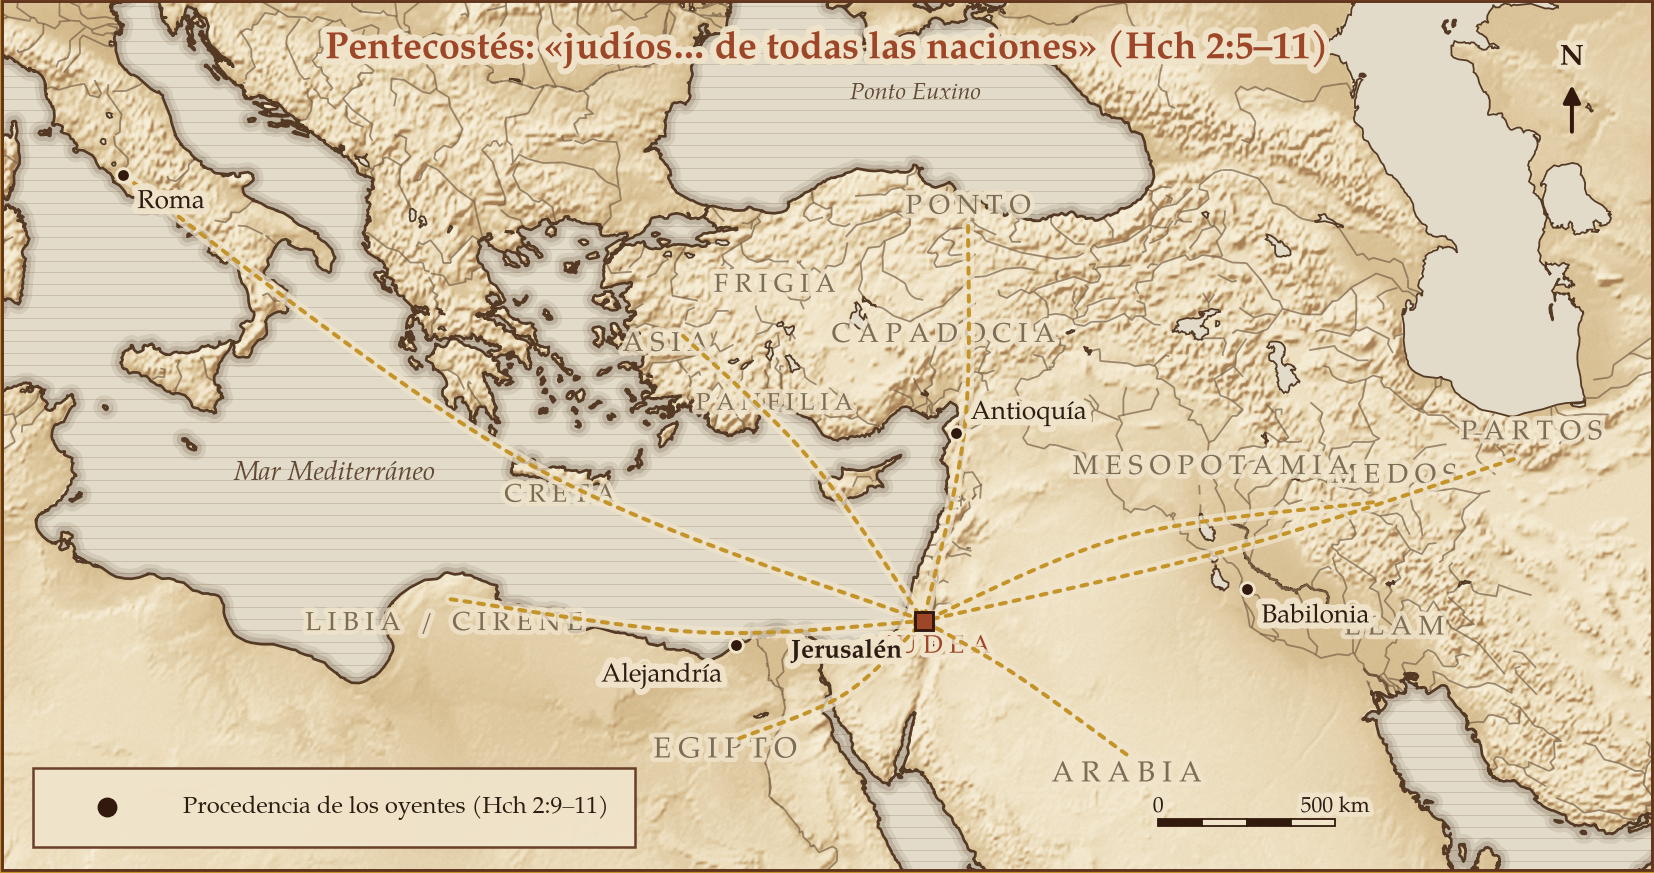
\includegraphics[width=\linewidth]{mapa_pentecostes.png}\\[4pt]
{\footnotesize\color{sepia}\RaggedRight\textit{Nota.} Elaboración propia: costas, lagos y ríos GSHHS/WDB y relieve sombreado (Basemap); ubicaciones antiguas aproximadas. Izquierda: la tierra de Israel en tiempos de Jesús y de la guerra; la huida a Pela es tradición discutida (Eusebio, HE 3.5.3). Derecha: procedencia de los oyentes de Pentecostés según Hch 2:9--11.\par}
\end{minipage}\end{center}

La fuente principal de la guerra es Josefo, sacerdote que comandó a los judíos en Galilea, se rindió en el 67 y escribió en Roma bajo patrocinio de los Flavios; es testigo directo, pero también apologista de Tito (Mason, 2016). La revuelta estalló en el 66, cuando se suspendieron los sacrificios ofrecidos por el emperador (\emph{Guerra} 2.409), y mientras Vespasiano sometía Galilea, las facciones se disputaban Jerusalén y quemaban sus reservas de grano (\emph{Guerra} 5.24--26). El templo ardió en Av del 70, el mismo día, observa Josefo, en que lo había quemado el rey de Babilonia (\emph{Guerra} 6.250). Su cifra de 1.100.000 muertos (\emph{Guerra} 6.420) excede cualquier estimación razonable de la población, y conviene darla siempre como «según Josefo». Tampoco la diáspora empezó entonces, pues existía desde el exilio babilónico (Hch 2:9--11). Masada resistió hasta el 73 o el 74.

La arqueología de la etapa es rica. Un osario hallado en 1990 lleva el nombre «Yehosef bar Qayafa», que muchos atribuyen al sumo sacerdote Caifás, aunque la lectura y la identificación se discuten (Evans, 2003). Una losa griega prohíbe a todo extranjero pasar la balaustrada del santuario bajo pena de muerte (\emph{Guerra} 5.193--194), dato que ilumina la «pared intermedia de separación» de Ef 2:14. Al pie de la explanada, los sillares caídos en el 70 sobre la calle herodiana dan contexto visual a Mt 24:2, «no quedará aquí piedra sobre piedra». En Masada, Yadin halló un rollo de Ezequiel 35--38, con la visión de los huesos secos, bajo el piso de la sinagoga (Yadin, 1966); el relato del suicidio colectivo procede solo de Josefo y su exactitud se discute (Ben-Yehuda, 1995).

\section{Desarrollo bíblico}

Pablo resume la venida de Jesús diciendo que «cuando vino la plenitud del tiempo, Dios envió a su Hijo, nacido de mujer, nacido bajo la ley» (Gá 4:4), y \grc{πλήρωμα} es la palabra con que hablará de la «plenitud» de Israel y de los gentiles (Ro 11:12, 25). Para Lucas esa venida cumple «el juramento que hizo a Abraham nuestro padre» (Lc 1:73). En el templo, Simeón, que esperaba la \grc{παράκλησιν τοῦ Ἰσραήλ} de Is 40:1, bendice a Dios con palabras del siervo:

\hebverso{לְהָקִים אֶת־שִׁבְטֵי יַעֲקֹב \foreignlanguage{spanish}{[\ldots]} וּנְתַתִּיךָ לְאוֹר גּוֹיִם לִהְיוֹת יְשׁוּעָתִי עַד־קְצֵה הָאָרֶץ}
\begin{cita}Poco es que tú me seas siervo para levantar las tribus de Jacob y para restaurar a los preservados de Israel; también te daré por luz de las naciones, para que seas mi salvación hasta el extremo de la tierra.\fuente{(Is 49:6)}\end{cita}
\begin{cita}Porque han visto mis ojos tu salvación [\ldots]: luz para revelación a las naciones y gloria de tu pueblo Israel.\fuente{(Lc 2:30--32)}\end{cita}

Simeón mantiene juntas \destacar{la gloria de Israel y la luz de las naciones}, aunque advierte que el niño está puesto «para caída y levantamiento de muchos en Israel» (2:34), vocabulario que Pablo retomará en Ro 11:11. Ana, «de la tribu de Aser», tribu del antiguo reino del norte (2:36), muestra que siglos después de la dispersión asiria las tribus de Jacob tienen quien las represente en el umbral del evangelio.

\subsection{Nazaret y las doce tribus}
En la sinagoga de Nazaret Jesús lee Is 61 y anuncia que «hoy se ha cumplido esta Escritura» (Lc 4:21). La libertad que proclama, \heb{דְּרוֹר} (\emph{derór}), es la del jubileo (Lv 25:10), cuando los cautivos vuelven y la tierra se restituye. El gesto más elocuente es la elección de los Doce:

\begin{cita}En la regeneración, cuando el Hijo del Hombre se siente en el trono de su gloria, vosotros que me habéis seguido os sentaréis también sobre doce tronos, para juzgar a las doce tribus de Israel.\fuente{(Mt 19:28)}\end{cita}

Dispersas las tribus del norte desde el 722 a.\,e.\,c., elegir a doce anunciaba la reconstitución de \emph{todo} Israel, conforme a Ez 37:15--28 (Sanders, 1985), y por eso los once completan el número antes de Pentecostés (Hch 1:15--26) y Santiago escribe «a las doce tribus que están en la dispersión» (Stg 1:1). La consigna de ir «a las ovejas perdidas de la casa de Israel» (Mt 10:6) evoca a su vez Ez 34, donde Dios promete reunir a las ovejas dispersas bajo «mi siervo David»; en Mateo esa casa es el pueblo judío entero de Galilea y Judea, no el antiguo reino del norte, pues a los Doce se les prohíbe entrar en Samaria.

\subsection{El templo, la viña y el lamento}
En el templo cita a Isaías, «mi casa, casa de oración será llamada» para todas las naciones (Is 56:7; Mc 11:17), y a Jeremías, «cueva de ladrones» (Jer 7:11), el sermón en que el profeta advirtió que Dios haría con el templo lo que hizo con Silo. Sobre la canción de la viña de Is 5, donde «la viña de YHWH de los ejércitos es la casa de Israel», construye la parábola de los labradores, que termina así:

\begin{cita}Por tanto os digo que el reino de Dios será quitado de vosotros y será dado a un pueblo que produzca sus frutos.\fuente{(Mt 21:43)}\end{cita}

El versículo se ha leído a menudo como traspaso del reino de Israel a la iglesia de los gentiles, pero el contexto lo resiste. Los destinatarios son los principales sacerdotes, que «entendieron que hablaba de ellos» (21:45); la viña no se destruye, sino que pasa «a otros labradores» (21:41), y Mateo escribe \grc{ἔθνει}, «a un pueblo», en singular, no «a los gentiles». Es un relevo en la conducción del pueblo de Dios hacia una comunidad judía en su núcleo.

El discurso de Mt 23 termina en llanto:

\begin{cita}¡Jerusalén, Jerusalén, que matas a los profetas [\ldots]! ¡Cuántas veces quise juntar a tus hijos, como la gallina junta a sus polluelos debajo de las alas, y no quisisteis! He aquí, vuestra casa os es dejada desierta. Porque os digo que desde ahora no me veréis, hasta que digáis: Bendito el que viene en el nombre del Señor.\fuente{(Mt 23:37--39)}\end{cita}

La casa desierta evoca Jer 22:5, pero el juicio tiene término: \grc{ἕως ἂν εἴπητε}, «\emph{hasta que} digáis», con la bienvenida de Sal 118:26, \heb{בָּרוּךְ הַבָּא בְּשֵׁם יְהוָה}. Allison (1983) mostró que la construcción expresa una condición: Jerusalén volverá a ver a Jesús cuando le dé la bienvenida. Lucas añade el anuncio del asedio:

\begin{cita}Caerán a filo de espada y serán llevados cautivos a todas las naciones; y Jerusalén será hollada por los gentiles, hasta que los tiempos de los gentiles se cumplan.\fuente{(Lc 21:24)}\end{cita}

El lenguaje es el de Dt 28:64 y de Jeremías sobre el 586, y la frase final, \grc{ἄχρι οὗ πληρωθῶσιν καιροὶ ἐθνῶν}, usa la misma construcción que Ro 11:25, donde el endurecimiento parcial dura \grc{ἄχρι οὗ τὸ πλήρωμα τῶν ἐθνῶν εἰσέλθῃ}. Qué sean esos «tiempos» se discute, pero la desolación tiene un plazo. La huida de los cristianos de Jerusalén a Pela que narra Eusebio (\emph{Historia eclesiástica} 3.5.3) coincide con Lc 21:21, aunque su historicidad se discute (Skarsaune y Hvalvik, 2007).

\subsection{El nuevo pacto y la pregunta por el reino}
En la cena de Pascua, Jesús toma la copa:

\hebverso{הִנֵּה יָמִים בָּאִים נְאֻם־יְהוָה וְכָרַתִּי אֶת־בֵּית יִשְׂרָאֵל וְאֶת־בֵּית יְהוּדָה בְּרִית חֲדָשָׁה}
\begin{cita}He aquí que vienen días, dice YHWH, en que haré un nuevo pacto con la casa de Israel y con la casa de Judá.\fuente{(Jer 31:31 [31:30])}\end{cita}

Al decir «esta copa es el nuevo pacto en mi sangre, que por vosotros se derrama» (Lc 22:20), Jesús retoma esa promesa. La LXX tradujo \heb{בְּרִית חֲדָשָׁה} por \grc{καινὴ διαθήκη}, y con el eco de «la sangre del pacto» de Éx 24:8 (Mt 26:28) Jesús sitúa su muerte entre el Sinaí y Jeremías. El doble nombre de Jer 31:31, la casa de Israel (el antiguo reino del norte) y la casa de Judá (el reino del sur), lleva implícita la reunificación de los dos reinos divididos desde 1~R 12 bajo un solo pacto escrito en el corazón. En la cruz, Juan cita Zac 12:10, «mirarán al que traspasaron» (Jn 19:37), el duelo de la casa de David que abre un manantial para la purificación (Zac 13:1). Resucitado, oye la pregunta de los discípulos:

\begin{cita}Señor, ¿restaurarás el reino a Israel en este tiempo? Y les dijo: No os toca a vosotros saber los tiempos o las sazones que el Padre puso en su sola potestad [\ldots].\fuente{(Hch 1:6--7)}\end{cita}

Jesús deja en pie el contenido de la pregunta y corrige solo el calendario. El verbo \grc{ἀποκαθιστάνεις} es el de Mal 3:23 [4:6] LXX, y la misión que les encarga recorre el mapa de Is 49:6: Jerusalén, Judea, Samaria, la región del antiguo reino del norte, y «hasta el extremo de la tierra» (Hch 1:8).

\subsection{El remanente creyente y la tienda de David}
El Espíritu es derramado en Shavuot sobre judíos «de todas las naciones bajo el cielo» (Hch 2:5), y entre ellos están los medos y los de Mesopotamia, adonde Asiria había deportado al reino del norte (2~R 17:6): para Lucas, Pentecostés inaugura la reunión del Israel disperso (Jervell, 1972). Siguen «una gran multitud de sacerdotes» (6:7) y las «decenas de miles» de judíos creyentes, «todos celosos por la ley», de los que Jacobo habla hacia el 57 (21:20). La iglesia de Jerusalén fue una comunidad judía que confesaba a Jesús como Mesías y guardaba la ley (Bauckham, 1995), el remanente en que la restauración ya había comenzado. Cuando llegan los gentiles, Jacobo responde con Amós, profeta en el reino del norte:

\hebverso{בַּיּוֹם הַהוּא אָקִים אֶת־סֻכַּת דָּוִיד הַנֹּפֶלֶת}
\begin{cita}Después de esto volveré y reedificaré la tienda de David, que está caída; [\ldots] para que el resto de los hombres busque al Señor, y todas las naciones sobre las cuales es invocado mi nombre.\fuente{(Hch 15:16--17; Am 9:11--12 LXX)}\end{cita}

La \emph{sukkat David} es la casa davídica caída tras la división y el exilio. Jacobo ve su reedificación en el Hijo de David resucitado y su fruto en la entrada de las naciones, que ingresan \emph{como gentiles}. Pablo, que predica «al judío primeramente» (Ro 1:16), habla también de un velo sobre la lectura de Moisés «hasta el día de hoy», que se quita «cuando se vuelva al Señor» (2~Co 3:14--16): el verbo \grc{ἐπωρώθη} comparte raíz con la \grc{πώρωσις ἀπὸ μέρους} de Ro 11:25, y \grc{ἐπιστρέφω} traduce en la LXX el hebreo \heb{שׁוּב}, el verbo del regreso.

\section{Israel como nación santa y reino de sacerdotes}

Mateo narra la infancia de Jesús como un nuevo recorrido de la historia de Israel. Tras la huida a Egipto cita, siguiendo el hebreo, Os 11:1, «de Egipto llamé a mi hijo», donde el hijo es el pueblo (Éx 4:22), y los cuarenta días del desierto responden a los cuarenta años: donde Israel murmuró, el Hijo confía. En Is 49 el siervo se llama «Israel» (49:3) y recibe, sin embargo, la misión de «hacer volver a Jacob» (49:5), tensión que solo se resuelve si el siervo encarna a Israel para restaurarlo; la tradición judía lo identificó con el pueblo o con el Mesías; el Nuevo Testamento reconoce en Jesús ambas cosas, de modo que el llamado de Éx 19:6 se cumple primero en una persona.

La vocación se vivió en el remanente, en judíos que llevaban el Mesías a las naciones, y Pablo describe su misión como un oficio sacerdotal (\grc{ἱερουργοῦντα}) «para que la ofrenda de las naciones sea aceptable» (Ro 15:16), eco de Is 66:20. Se quebró en la dirigencia del templo y en una ciudad cuyas facciones mataban a otros judíos en los atrios, y se preservó en el remanente creyente y en el judaísmo rabínico, que custodió la Torá cuando cayó el templo (Ro 3:2). Los gentiles, por su parte, entran en la «ciudadanía de Israel» (Ef 2:12) y se alegran «con su pueblo» (Ro 15:10; Dt 32:43 LXX), y 1~P 2:9--10 les comparte los títulos de Éx 19:6 junto con la promesa de Os 1:10 [2:1] al reino del norte, «no mi pueblo» llamado a ser pueblo de Dios, sin que Israel los pierda.

\section{Aporte de la tradición judía}

La tradición rabínica, escrita entre los siglos \textsc{ii} y \textsc{vi}, no es un relato histórico verificado. Según el Talmud, Yohanán ben Zakai salió de Jerusalén sitiada en un ataúd y pidió a Vespasiano «Yavne y sus sabios» (Guitín 56a--b), y allí se reorganizó la vida judía sin templo. Cuando su discípulo lloró la pérdida del lugar de la expiación, Yohanán respondió que quedaban los actos de bondad, \emph{gemilut jasadim}, «como está dicho: \emph{Porque misericordia quiero y no sacrificio}» (Os 6:6; Avot de-Rabí Natán 4), el versículo que Jesús había citado dos veces (Mt 9:13; 12:7). El Talmud atribuye la caída del Segundo Templo al \heb{שִׂנְאַת חִנָּם}, el odio gratuito entre hermanos, que «equivale a las tres transgresiones» de idolatría, inmoralidad y sangre que destruyeron el Primero (Yoma 9b), una autocrítica que concuerda con las facciones de Josefo. La Mishná fija la memoria el 9 de Av, cuando «fue destruida la casa la primera y la segunda vez» (Taanit 4:6); ese día se ayuna y se lee Lamentaciones, pero el sábado siguiente se llama \emph{Shabat Najamú} por Is 40:1, «Consolad, consolad a mi pueblo», el consuelo que esperaba Simeón. Sin altar, la oración ocupó el lugar del sacrificio (Berajot 26b), y la Amidá incorporó la petición diaria por la reconstrucción de Jerusalén (Sacks, 2009).

\section{La promesa de restauración}

Isaías y Jeremías dan a esta etapa sus textos de restauración. El Redentor de Isaías viene precisamente a la ciudad que el año 70 deja en ruinas:

\hebverso{וּבָא לְצִיּוֹן גּוֹאֵל וּלְשָׁבֵי פֶשַׁע בְּיַעֲקֹב נְאֻם יְהוָה}
\begin{cita}Y vendrá el Redentor a Sion, y a los que se vuelvan de la rebelión en Jacob, dice YHWH.\fuente{(Is 59:20)}\end{cita}

La liturgia judía abre con él la oración diaria \emph{U-va le-Tsiyón}, y Pablo lo citará en Ro 11:26. Jeremías, cuyo sermón del templo y cuyo nuevo pacto resuenan en Jesús, ató la permanencia de Israel al orden del cosmos cuando Jerusalén estaba por caer ante Babilonia: si faltaran las leyes del sol y la luna, «también la descendencia de Israel faltará para no ser nación delante de mí para siempre» (Jer 31:36 [31:35]). La Torá ya había previsto ese juicio dentro del pacto (Lv 26:44). Los textos del Nuevo Testamento que anuncian el juicio le fijan, a su vez, un límite:

\begin{center}\small
\renewcommand{\arraystretch}{1.2}
\begin{tabular}{>{\RaggedRight\arraybackslash}p{2.2cm}>{\RaggedRight\arraybackslash}p{4.6cm}>{\RaggedRight\arraybackslash}p{7.1cm}}
\toprule
\textbf{Texto} & \textbf{Expresión griega} & \textbf{Lo que termina}\\
\midrule
Mt 23:39 & \grc{ἕως ἂν εἴπητε} & La ausencia del Mesías para Jerusalén, cuando diga: «Bendito el que viene»\\
Lc 21:24 & \grc{ἄχρι οὗ πληρωθῶσιν} & La Jerusalén hollada, cuando se cumplan los tiempos de los gentiles\\
Hch 1:6--7 & \grc{ἐν τῷ χρόνῳ τούτῳ} & La pregunta por el reino: no se niega; se remite al tiempo del Padre\\
Hch 3:21 & \grc{ἄχρι χρόνων ἀποκαταστάσεως} & El Mesías en el cielo, hasta la restauración de todas las cosas\\
2~Co 3:14--16 & \grc{ἄχρι τῆς σήμερον ... ἡνίκα ἐάν} & El velo, cuando Israel se vuelva al Señor\\
Ro 11:25 & \grc{ἄχρι οὗ ... εἰσέλθῃ} & El endurecimiento parcial, cuando entre la plenitud de los gentiles (Estudio 8)\\
\bottomrule
\end{tabular}\end{center}

El más explícito es el discurso de Pedro a los «varones israelitas» en el pórtico de Salomón:

\begin{cita}Así que, arrepentíos y volveos, para que sean borrados vuestros pecados, para que vengan de la presencia del Señor tiempos de refrigerio, y él envíe al Mesías que os fue anunciado, Jesús, a quien es necesario que el cielo reciba hasta los tiempos de la restauración de todas las cosas, de que habló Dios por boca de sus santos profetas.\fuente{(Hch 3:19--21)}\end{cita}

La \grc{ἀποκατάστασις} retoma el verbo de Hch 1:6 y apunta a lo que anunciaron los profetas, y Pedro recuerda a sus oyentes que son «hijos [\ldots] del pacto que Dios hizo con nuestros padres, diciendo a Abraham: En tu simiente serán benditas todas las familias de la tierra» (3:25). Pablo, hacia el 57, pregunta: «¿Ha desechado Dios a su pueblo? ¡De ninguna manera! Porque también yo soy israelita» (11:1). Funda su respuesta no en la suerte política de Jerusalén sino en el carácter de Dios: «irrevocables son los dones y el llamamiento de Dios» (\grc{ἀμεταμέλητα}, 11:29). ONE FOR ISRAEL (2025) llega a la misma conclusión: en el siglo \textsc{i} hubo un remanente numeroso, aunque la mayoría no creyó, y la palabra clave de Romanos 11 y de Lc 21:24 es «hasta».

\section{Conclusión y puente al Estudio 8}

En esta etapa Jesús aparece como el Mesías \emph{de Israel}: asume el llamado de su pueblo como Hijo y como siervo, elige a doce para anunciar la reunión de todas las tribus y establece el nuevo pacto prometido a la casa de Israel y a la casa de Judá. Un remanente judío creyente forma el núcleo del pueblo restaurado, y las naciones entran por la tienda reedificada de David sin desplazarlo. El templo cayó en un juicio anunciado con palabras de Jeremías, y la tradición judía respondió con la Torá, la oración y los actos de bondad. Pero ese juicio lleva inscrito su límite en los «hasta» de Mt 23:39, Lc 21:24 y Hch 3:21, y la palabra de Pablo en Ro 11:1 y 29 impide leer el año 70 como rechazo definitivo: como el 586 para Jeremías, fue el escenario en que la promesa de restauración se renovó.

Queda la pregunta que Pablo plantea en Romanos 9--11: si Israel en su mayoría no reconoció al Mesías, ¿qué será de él? Pablo responde con un remanente escogido por gracia, un olivo cuyas ramas naturales pueden ser injertadas de nuevo y un misterio: «y así todo Israel será salvo» (Ro 11:26). Ese es el tema del Estudio~8, \emph{Romanos 11: la restauración de Israel}, que reunirá los hilos de toda la serie.

\section*{Preguntas para la reflexión}\markboth{Preguntas para la reflexión}{}
\begin{enumerate}
\item Simeón une «luz para las naciones» y «gloria de tu pueblo Israel» (Lc 2:32). ¿Qué se pierde cuando la iglesia se queda solo con la primera mitad del versículo?
\item ¿Qué importancia tiene que Mt 21:43 hable de los dirigentes y de «un pueblo» en singular?
\item ¿Qué «hasta» de esta etapa le parece más significativo para la esperanza de Israel, y por qué?
\end{enumerate}

\section*{Glosario}\markboth{Glosario}{}
\begin{description}\small
\item[Apokatástasis] (\grc{ἀποκατάστασις}). Restauración. «Hasta los tiempos de la restauración de todas las cosas» (Hch 3:21); verbo en Hch 1:6.
\item[Brit jadashá] (\heb{בְּרִית חֲדָשָׁה}). Nuevo pacto (Jer 31:31 [31:30]); en griego \grc{καινὴ διαθήκη} (Lc 22:20).
\item[Gemilut jasadim] (\heb{גְּמִילוּת חֲסָדִים}). Actos de bondad. Según Yohanán ben Zakai, expiación que sustituye al sacrificio (Os 6:6).
\item[Kairoí ethnōn] (\grc{καιροὶ ἐθνῶν}). «Tiempos de los gentiles» (Lc 21:24), plazo al que está sujeta la Jerusalén hollada.
\item[Pórosis] (\grc{πώρωσις}). Endurecimiento. «Endurecimiento en parte» (Ro 11:25); el verbo en 2~Co 3:14.
\item[Sinat jinam] (\heb{שִׂנְאַת חִנָּם}). Odio gratuito. Causa de la destrucción del Segundo Templo según Yoma 9b.
\item[Sukkat David] (\heb{סֻכַּת דָּוִיד}). «Tienda de David», la casa davídica caída que Dios levantará (Am 9:11; Hch 15:16).
\end{description}

\section*{Referencias}\markboth{Referencias}{}
\refapa{Allison, D.~C., Jr. (1983). Matt. 23:39 = Luke 13:35b as a conditional prophecy. \emph{Journal for the Study of the New Testament, 5}(18), 75--84.}
\refapa{Bauckham, R. (1995). James and the Jerusalem church. En R. Bauckham (Ed.), \emph{The book of Acts in its Palestinian setting}. Eerdmans.}
\refapa{Ben-Yehuda, N. (1995). \emph{The Masada myth: Collective memory and mythmaking in Israel}. University of Wisconsin Press.}
\refapa{\emph{Biblia Hebraica Stuttgartensia} (5.ª ed.). (1997). Deutsche Bibelgesellschaft.}
\refapa{Danby, H. (Trad.). (1933). \emph{The Mishnah}. Oxford University Press.}
\refapa{Epstein, I. (Ed.). (1935--1948). \emph{The Babylonian Talmud}. Soncino Press.}
\refapa{Eusebio de Cesarea. (1926). \emph{The ecclesiastical history} (K. Lake, Trad.; Vol. 1). Harvard University Press.}
\refapa{Evans, C.~A. (2003). \emph{Jesus and the ossuaries}. Baylor University Press.}
\refapa{Jervell, J. (1972). \emph{Luke and the people of God: A new look at Luke-Acts}. Augsburg.}
\refapa{Josefo, F. (1987). \emph{The works of Josephus} (W. Whiston, Trad.). Hendrickson.}
\refapa{Mason, S. (2016). \emph{A history of the Jewish War, A.D. 66--74}. Cambridge University Press.}
\refapa{\emph{Novum Testamentum Graece} (28.ª ed.). (2012). Deutsche Bibelgesellschaft.}
\refapa{ONE FOR ISRAEL Ministry. (2025, 3 de julio). \emph{What does «all Israel will be saved» mean in Romans 11?} \url{https://www.oneforisrael.org/what-does-all-israel-will-be-saved-mean-in-romans-11/}}
\refapa{Rahlfs, A., \& Hanhart, R. (Eds.). (2006). \emph{Septuaginta} (ed. rev.). Deutsche Bibelgesellschaft.}
\refapa{Sacks, J. (Trad.). (2009). \emph{The Koren Siddur}. Koren Publishers.}
\refapa{Sanders, E.~P. (1985). \emph{Jesus and Judaism}. Fortress Press.}
\refapa{Skarsaune, O., \& Hvalvik, R. (Eds.). (2007). \emph{Jewish believers in Jesus: The early centuries}. Hendrickson.}
\refapa{Yadin, Y. (1966). \emph{Masada: Herod's fortress and the Zealots' last stand}. Random House.}
\end{document}
